% % % % % % % % % % % % % % % % % % % % % % % % % % % % % % % % % % % % % % % % % % % %
%                                                                                     %
% Short Sectioned Assignment LaTeX Template Version 1.0 (5/5/12)                      %
% This template has been downloaded from: http://www.LaTeXTemplates.com               %
%                                                                                     %
% Original author:  Frits Wenneker (http://www.howtotex.com)                          %
%                                                                                     %
% Modified by: Fco Javier Sueza Rodríguez (fcosueza@disroot.org)                      %
%                                                                                     %
% Changes:                                                                            %
%	    - Custom Chapters, Sections and Subsections (titlesec package)                %
%           - Document type scrbook (oneside)                                         %
%           - Use babel-lang-spanish package and marvosym                             %
%           - Use hyperref, enumitem, tcolorbox and glossaries packages               %
%           - Use Time New Roman (mathptmx), Helvetic and Courier fonts               %
%                                                                                     %
% License: CC BY-NC-SA 3.0 (http://creativecommons.org/licenses/by-nc-sa/3.0/)        %
%                                                                                     %
% % % % % % % % % % % % % % % % % % % % % % % % % % % % % % % % % % % % % % % % % % % %

%-----------------------------------------------%
%	              Packages                  %
%-----------------------------------------------%

\documentclass[paper=a4, fontsize=11pt, oneside]{scrbook}

% ---- Text Input/Output ----- %

\usepackage[T1]{fontenc}
\usepackage[utf8]{inputenc}
\usepackage{mathptmx}
\usepackage[scaled=.92]{helvet}
\usepackage{courier}
\usepackage[indent=12pt]{parskip}

\usepackage{geometry}
\geometry{verbose,tmargin=3cm,bmargin=3cm,lmargin=2.6cm,rmargin=2.6cm}

% ---- Language ----- %

\usepackage[spanish]{babel}
\usepackage{marvosym}

% ---- Another packages ---- %

\usepackage{amsmath,amsfonts,amsthm}
\usepackage{graphics,graphicx}
\usepackage{titlesec}
\usepackage{fancyhdr}
\usepackage{tcolorbox}
\usepackage{hyperref}
\usepackage{enumitem}
\usepackage[automake]{glossaries}

%--------------------------------------------------------------------%
%                      Customizing Document                          %
%--------------------------------------------------------------------%


% ----------- Custom Chapters, Sections and Subsections -------------- %

\titleformat{\chapter}[display]
			{\bfseries\Huge}
			{Tema \ \thechapter} {0.5ex}
			{\vspace{1ex}\centering}

\titleformat{\section}[hang]
			{\bfseries\Large}
			{\thesection}{0.5em}{}

\titleformat{\subsection}[hang]
			{\bfseries\large}
			{\thesubsection}{0.5em}{}

\titleformat{\subsubsection}[hang]
			{\bfseries\large}
			{\thesubsubsection}{0.5em}{}

\hypersetup{
    colorlinks=true,
    linkcolor=black,
    urlcolor=magenta
}

% ------------------- Custom heaaders and footers ------------------- %

\pagestyle{fancyplain}

\fancyhead[]{}
\fancyfoot[L]{}
\fancyfoot[C]{}
\fancyfoot[R]{\thepage}

\renewcommand{\headrulewidth}{0pt} % Remove header underlines
\renewcommand{\footrulewidth}{0pt} % Remove footer underlines

\setlength{\headheight}{13.6pt} % Customize the height of the header

% --------- Numbering equations, figures and tables ----------------- %

\numberwithin{equation}{section} % Number equations within sections
\numberwithin{figure}{section} % Number figures within sections
\numberwithin{table}{section} % Number tables within sections

% ------------------------ New Commands ----------------------------- %

\newcommand{\horrule}[1]{\rule{\linewidth}{#1}} % Create horizontal rule command


%----------------------------------------------------------------------------------------
%	TÍTULO Y DATOS DEL ALUMNO
%----------------------------------------------------------------------------------------

\title{
\vspace{10ex}
\normalfont \normalsize
\huge \textbf{Tarea 1: Arquitecturas y Lenguajes de Programación en Clientes Web}
}
\author{Francisco Javier Sueza Rodríguez}
\date{\normalsize\today}

%----------------------------------------------------------------------------------------
%                                     DOCUMENTO
%----------------------------------------------------------------------------------------
\begin{document}

\maketitle

\thispagestyle{empty}

\vspace{65ex}

\begin{center}
    \begin{tabular}{l l}
        \textbf{Centro}: & IES Aguadulce \\
        \textbf{Ciclo Formativo}: & Desarrollo Aplicaciones Web (Distancia)\\
        \textbf{Asignatura}: & Desarrollo Web en Entorno Cliente\\
        \textbf{Tema}: & Tema 1 -  Arquitecturas y Lenguajes de Programación en Clientes Web\\
    \end{tabular}
\end{center}

\newpage

\section{Ejercicio 1}

\subsection{Enunciado}
Elige  e instala en tu sistema operativo al menos 2 navegadores web (adicionales al que ya tienes instalado por defecto). Por ejemplo, si ya tienes instalado Firefox instala otros dos más.

Deben realizarse capturas autenticables del proceso de instalación.  Autenticable es que aparezca tu usuario de distancia y la web en algún lado en otro navegador

\subsection{Solución}
En este ejercicio se van a instalar 2 navegadores adicionales a los que ya hay instalados en el sistema operativo. En mi caso, ya tengo instalados \textbf{Chrome}, \textbf{Mozilla Firefox Developer Edition}, mi navegador principal, y \textbf{Konqueror}, el viene por defecto con KDE. Además, también esta instalado \href{https://es.wikipedia.org/wiki/Links}{Links}, un navegador en modo texto para consola, pero que no soporta Javascript. Para esta actividad se van a instalar \textbf{Opera} y \textbf{Vivaldi}.

La instalación de \textbf{Opera} se va a realizar mediante la aplicación Discover de Kubuntu. Opera es un navegador creado por la empresa noruega Opera Software, compatible en un inicio solo con MS Windows, actualmente es además compatible con macOS y GNU-Linux entre otros. En la siguiente captura vemos su proceso de instalación.

Actualmente opera usa el motor \textbf{Blink} y el intérprete de JS \textbf{V8}.

\begin{figure}[H]
    \centering
    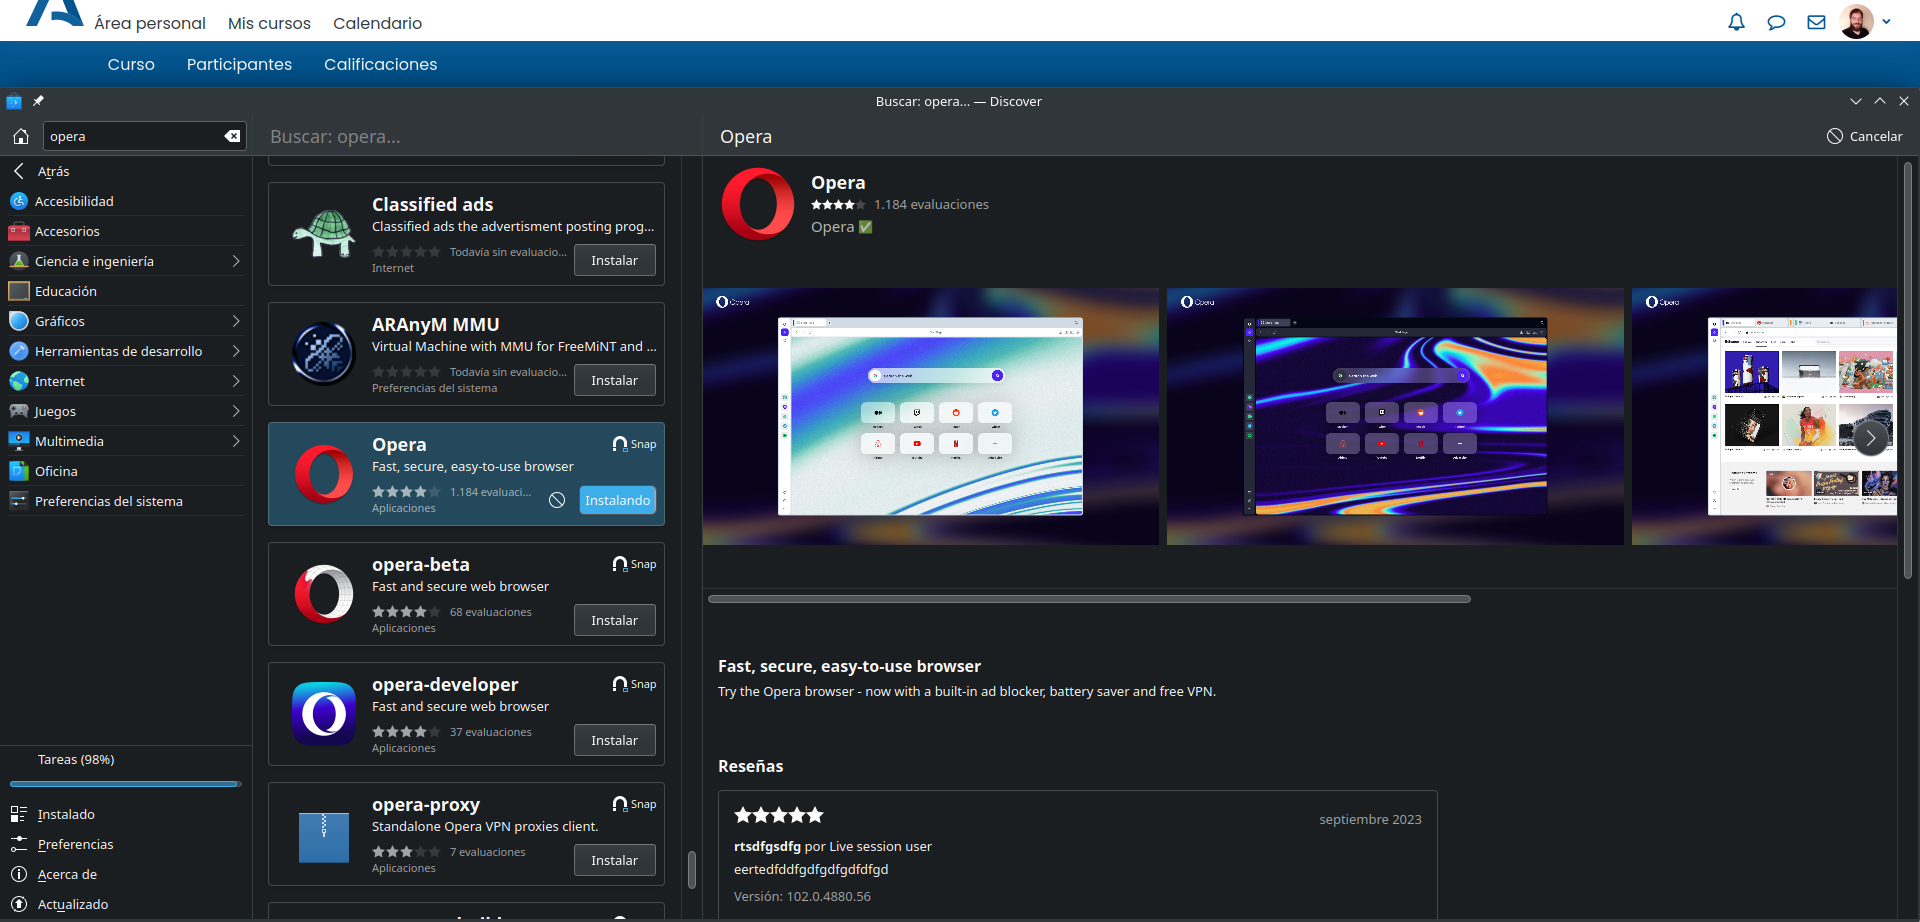
\includegraphics[scale=0.32]{instalacion-opera.png}
\end{figure}

\textbf{Vivaldi} es un fork de Opera que fue desarrollado por Jon Stephenson von Tetzchner, que más tarde fundaría Vivaldi Technologies, empresa que actualmente se encarga del desarrollo y mantenimiento del navegador. Para instalarlo se ha descargado el paquete para Ubuntu (.deb) y se ha instalado usando el gestor de paquetes, como se ve en la siguiente captura.

Aunque en un principio mantuvo el motor HTMl \textbf{Presto} y el interprete JS \textbf{Carakan} que tenía originalmente Opera, actualmente también ha realizado la transición a \textbf{Blink} y \textbf{V8}.

\begin{figure}[H]
    \centering
    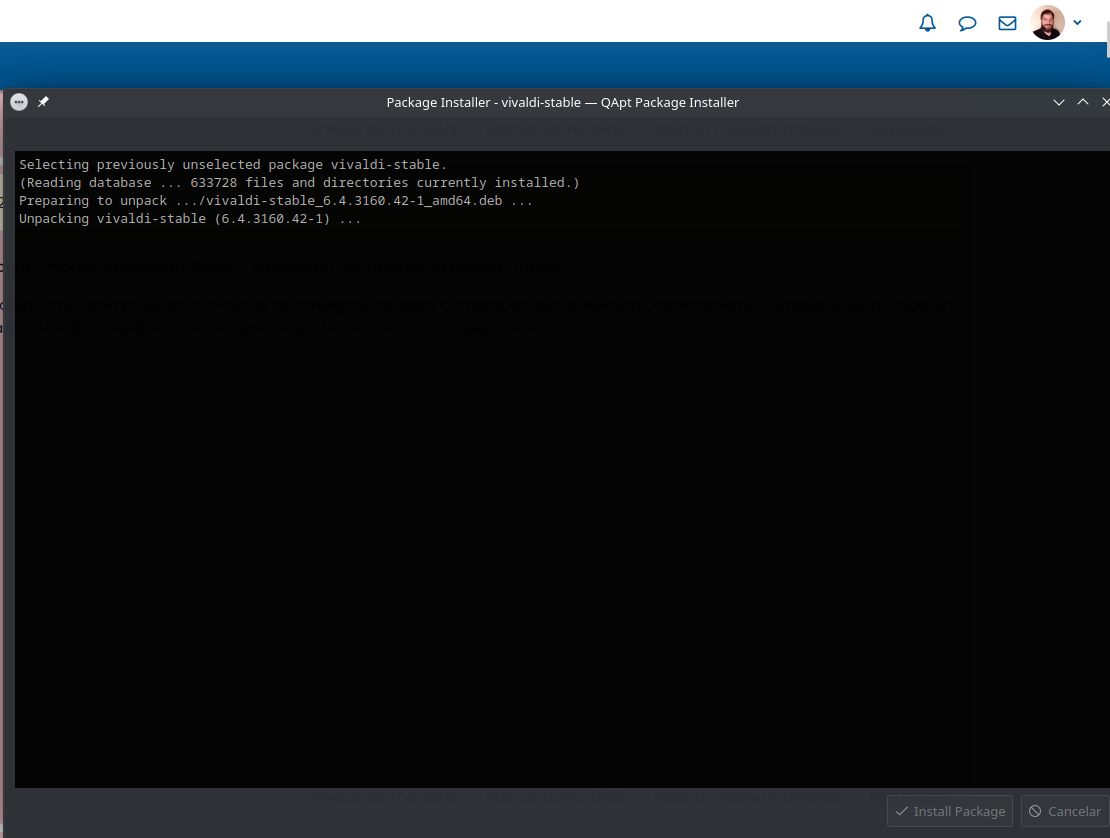
\includegraphics[scale=0.52]{instalacion-vivaldi.png}
\end{figure}

\section{Ejercicio 2}
\subsection{Enunciado}
¿Por qué es conveniente tener instalados al menos dos navegadores diferentes en tu ordenador? Se abrirá un hilo en el foro. Comente ahí.   Indica el nombre del motor HTML y JavaScript de los navegadores que has instalado.

\subsection{Solución}
A continuación se muestra la captura con la intervención en el foro respondiendo a la pregunta que se nos hace en el enunciado.

\begin{figure}[H]
    \centering
    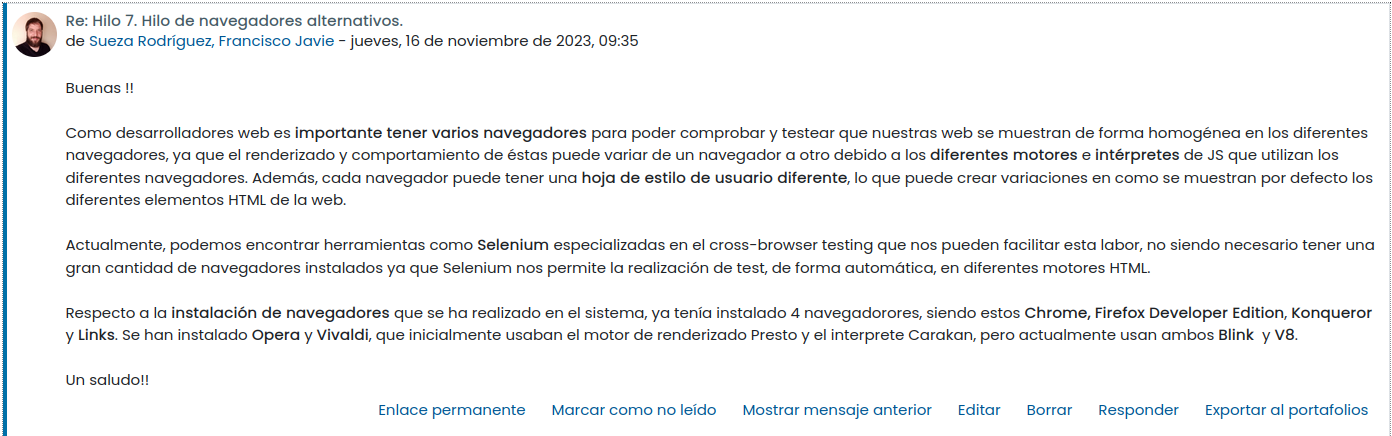
\includegraphics[scale=0.45]{foro-1.png}
\end{figure}

\section{Ejercicio 3}
\subsection{Enunciado}
¿Ves conveniente que  Firefox abandone su motor y use blink?  Existirá un hilo en el foro. No abra el suyo. Realiza una captura de tu intervención y añádela al documento.  Entre en el hilo específico que se ha abierto en el foro  y haz un comentario sobre navegadores independientes. Realiza una captura de tu intervención y añádela al documento.

\subsection{Solución}
En la siguiente imagen, podemos ver la intervención en el foro respondiendo a la pregunta que se nos realizad enunciado de este ejercicio.

\begin{figure}[H]
    \centering
    
\includegraphics[scale=0.45]{foro-2.png}
\end{figure}

\section{Ejercicio 4}
\subsection{Enunciado}
Elige un editor para JavaScript e instálalo.  En los materiales y en los foros hay ejemplos de  editores JavaScript. Debes realizar una tabla comparativa de características para sustentar tu opinión. Si no la haces tendrás un 0 en este apartado.


\subsection{Solución}
El editor elegido para su instalación ha sido \textbf{VS Code}. También se ha valorado el uso de Netbeans, pero después de usar ambos editor y ver sus características se ha optado por VS Code. En la siguiente liste podemos ver las características que me han hecho decantarme por VS Code sobre Netbeans:

\begin{itemize}
    \item \textbf{Netbeans}:
           \begin{itemize}
               \item \textbf{Lenguaje Principal}: Java
               \item \textbf{Soporte Plugins}: Si
               \item \textbf{Soporte JS}: Soporte nativo para Javascript.
               \item \textbf{Resalte de Sintaxis}: Si
               \item \textbf{Incluye Debugger para JS}: No
               \item \textbf{Autocompletado de Código}: Si, de forma nativa aunque el funcionamiento es un poco engorroso y la configuración por defecto no es la idónea.
               \item \textbf{Soporte para Prettier}: Plugin genérico para formateadores externos (peor integrado)
               \item \textbf{Rendimiento}: Netbeans es un IDE bastante pesado con un consumo bastante algo, especialmente de memoria RAM.
           \end{itemize}

    \item \textbf{VS Code}:
          \begin{itemize}
              \item \textbf{Lenguaje Principal}: Multilenguaje
              \item \textbf{Soporte de Plugins}: Si
              \item \textbf{Suporte JS}: Soporte nativo para Javascript.
              \item \textbf{Resalte de Sintaxis}: Si
              \item \textbf{Incluye Debugger para JS}: Si, incluye debugger para JS, TS y Node.
              \item \textbf{Autocompletado de Código}: Si, mediante intellisense, bastante más intuitivo y rápido, que el autocompletado nativo proporcionado por Netbeans.
              \item \textbf{Soporte para Prettier}: Plugin específico de prettier (mejor integración)
              \item \textbf{Rendimiento}: VS Code es un IDE muy ligero con muy buen rendimiento.
          \end{itemize}
\end{itemize}

En definitiva, se ha \textbf{elegido VS Code} porque tiene \textbf{mejor rendimiento}, especialmente en mi portátil que tiene una cantidad de memoria RAM bastante baja.

Además, la \textbf{integración de las diferentes aplicaciones} usadas en la cadena de herramientas para el desarrollo de JS es mucho \textbf{mejor en VS Code} que en Netbeans. Aplicaciones como prettier, eslint, code climate, etc.., tienen plugins específicos para VS Code, así como otras funcionalidades que permiten visualización de la web generada en una pestaña, edición multilínea de forma mas intuitiva, mejor integración con Emmet, etc.

\section{Ejercicio 5}
\subsection{Enunciado}
Para finalizar, usando la dirección de validación del W3C indicada en los apuntes, realiza la validación de la página de contenido informático \href{https://slashdot.org/}{Slashdot}. Indica la solución solamente a 3 problemas diferentes.

\subsection{Solución}
Se ha usado la página de validación de la W3C con la página de noticias \textbf{Slashdot}. El validador de la W3C a mostrado varios errores, de los cuales vamos a proponer aquí la solución a 3 de ellos, que son los siguientes:

\begin{enumerate}
    \item \textbf{Warning}: Content-Security-Policy HTTP header: Bad content security policy: Source list contains duplicate source expression "slashdot.org". All but the first instance will be ignored.

    \textbf{Solución}: Este error nos dice que hay duplicados en los elementos que definen la política segura de contenido en la cabecera HTML. Para solucionarlo, bastaría con eliminar los elementos duplicados.

    \item \textbf{Error}: A meta element with an http-equiv attribute whose value is X-UA-Compatible must have a content attribute with the value IE=edge.

    \textbf{Solución}: Este error nos dice que hay un elemento meta en la cabecera de tipo http-equiv al que le falta el atributo \textit{content} con el valor ``IE=edge''. Como podemos ver en el error, dicho atributo existe, con el valor ``IE=edge, chrome=1'', por lo que podríamos eliminar el segundo valor, chrome=1, para subsanar este error,

    \item \textbf{Warning}: The type attribute is unnecessary for JavaScript resources.

    \textbf{Solución}: aquí se nos muestra un advertencia, especificando que el atributo \textit{type} no es necesario para los recursos Javascript. Eliminando este atributo en la etiqueta \textit{script} podríamos eliminar este error.
\end{enumerate}

En la siguiente captura, podemos ver el resultado del validador de la W3C, donde además, se muestran los 3 errores que hemos comentado en la lista anterior.

\begin{figure}[H]
    \centering
    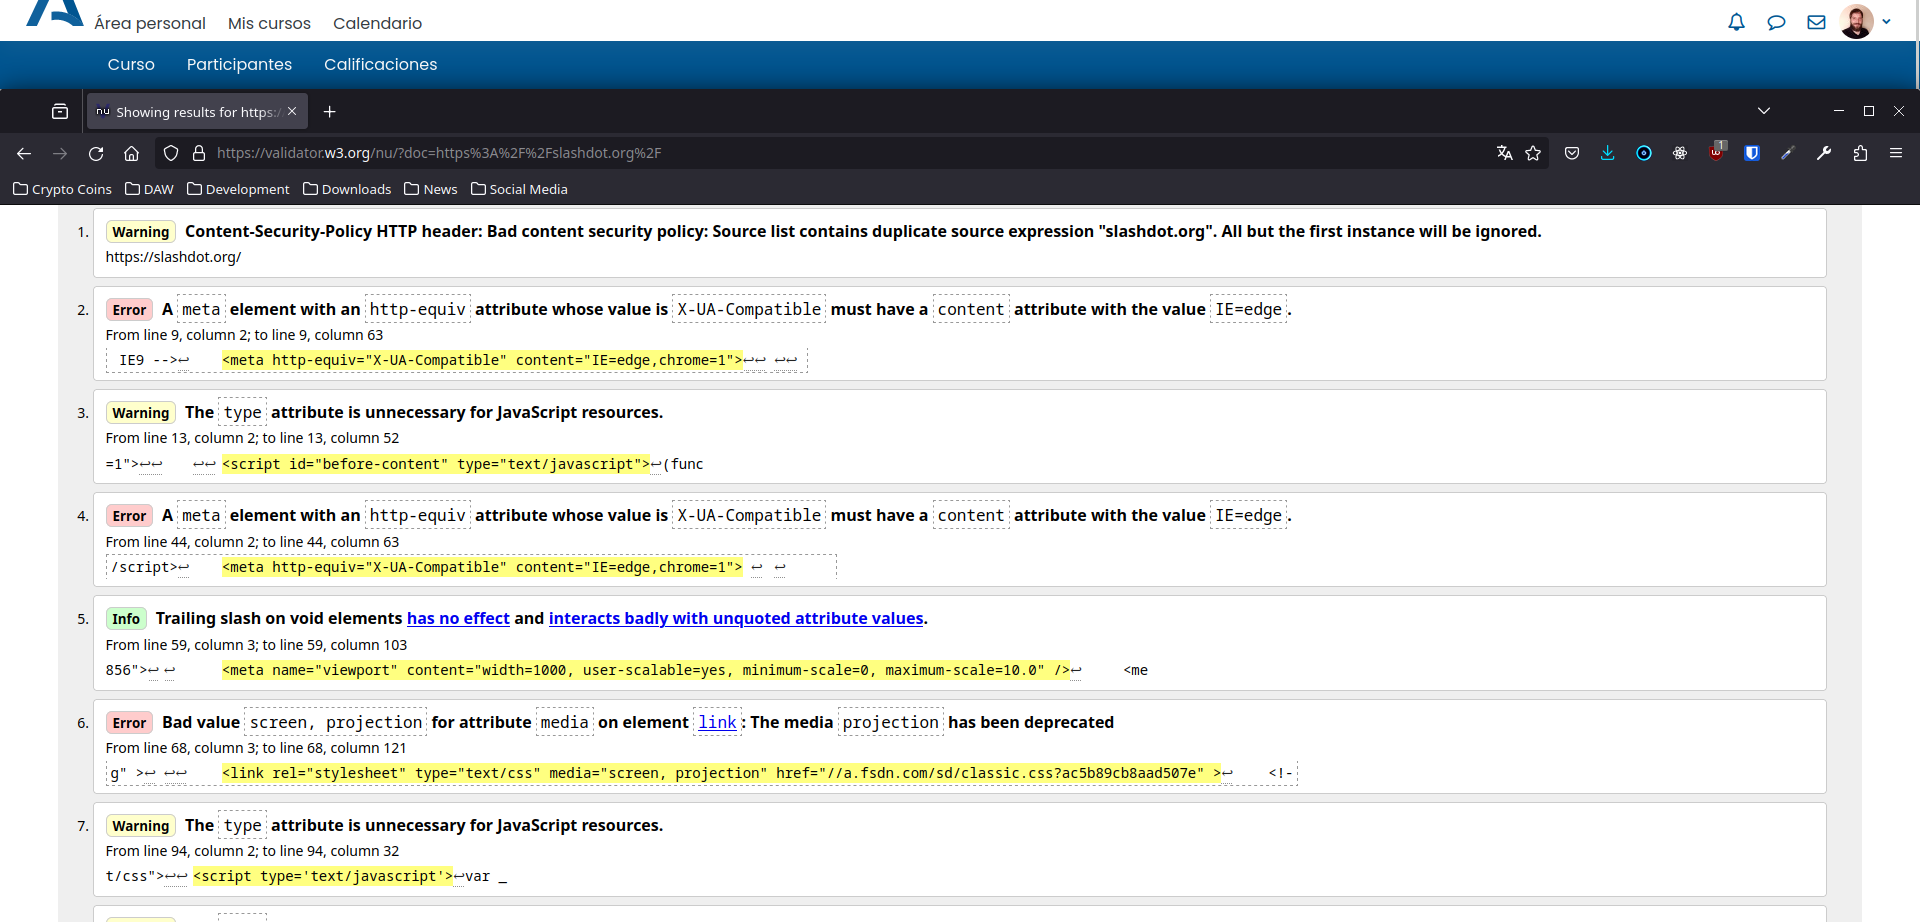
\includegraphics[scale=0.30]{validador.png}
\end{figure}



% Bibliography

%\newpage
%\bibliography{citas}
%\bibliographystyle{unsrt}

\end{document}